\begin{frame}{Tổng quan các phương pháp phát hiện té ngã}
\scriptsize
\begin{tabular}{|p{0.18\linewidth}|p{0.22\linewidth}|p{0.25\linewidth}|p{0.25\linewidth}|}
\hline
\textbf{Phương pháp} & \textbf{Cơ chế} & \textbf{Ưu điểm} & \textbf{Nhược điểm} \\
\hline
Đeo được & IMU (gia tốc kế, con quay hồi chuyển); phát hiện gia tốc/tư thế bất thường & Phản hồi nhanh; chính xác; chi phí thấp & Cần đeo liên tục; dễ false positive; pin/hiệu chuẩn \\
\hline
Môi trường & Cảm biến cố định: sàn áp suất, PIR, âm thanh; AI phân tích & Không xâm phạm; giám sát nhiều người; tích hợp smart home & Chi phí cao; phạm vi hạn chế; nhầm vật thể \\
\hline
Thị giác & Camera RGB/RGB-D/IR; pose estimation (OpenPose/MediaPipe) & Thông tin trực quan; không cần đeo; tích hợp giám sát & Quyền riêng tư; phụ thuộc ánh sáng; cần phần cứng mạnh \\
\hline
Đa phương thức & Kết hợp IMU + camera + môi trường; data fusion (Kalman/Deep Learning) & Độ chính xác cao; giảm cảnh báo sai; mở rộng phạm vi; kinh tế & Phức tạp; tốn năng lượng; đồng bộ khó \\
\hline
\end{tabular}

\vspace{0.3em}
\begin{itemize}\scriptsize
    \item Kết hợp dữ liệu để xác nhận té ngã, giảm false positive.  
    \item Chế độ linh hoạt: In-situ (cục bộ) + Mobile (edge device).  
    \item Bảo mật: xử lý cục bộ, chỉ gửi dữ liệu tối thiểu, tùy chỉnh khu vực nhạy cảm.
\end{itemize}
\end{frame}
% Slide 1: Tổng quan
\begin{frame}
\frametitle{Các Giao Thức Truyền Thông trong Hệ Thống Cảnh Báo IoT}
\begin{center}
\Large Hệ thống phát hiện ngã với ba giao thức cốt lõi
\end{center}

\begin{itemize}
\item \textbf{SIP}: Truyền tải âm thanh/video cảnh báo thời gian thực
\item \textbf{MQTT}: Vận chuyển dữ liệu cảm biến từ thiết bị IoT  
\item \textbf{JSON}: Định dạng cấu trúc dữ liệu trao đổi
\end{itemize}

\begin{block}{Mục tiêu}
Xây dựng hệ thống cảnh báo không gián đoạn, độ trễ thấp từ cảm biến đến cuộc gọi VoIP
\end{block}
\end{frame}

% Slide 2: Giao thức SIP
\begin{frame}
\frametitle{Giao thức SIP - Khởi tạo Phiên}

\textbf{Chức năng chính:}
\begin{itemize}
\item Thiết lập cuộc gọi VoIP từ hệ thống cảnh báo
\item Kết nối với Asterisk PBX để gọi điện thoại
\item Truyền âm thanh cảnh báo qua RTP
\end{itemize}

\textbf{Các bước hoạt động:}
\begin{enumerate}
\item REGISTER: Đăng ký thiết bị với server
\item INVITE: Khởi tạo cuộc gọi cảnh báo
\item ACK: Xác nhận kết nối thành công
\item RTP: Truyền dữ liệu âm thanh
\item BYE: Kết thúc cuộc gọi
\end{enumerate}

\begin{alertblock}{Lưu ý}
Sử dụng ICE để xuyên NAT, TLS/SRTP để bảo mật
\end{alertblock}
\end{frame}

% Slide 3: Giao thức MQTT
\begin{frame}
\frametitle{Giao thức MQTT - Truyền Dữ Liệu Cảm Biến}

\textbf{Đặc điểm:}
\begin{itemize}
\item Nhẹ, tiết kiệm băng thông cho thiết bị IoT
\item Mô hình Publish/Subscribe qua Broker
\item Hỗ trợ 3 mức QoS đảm bảo độ tin cậy
\end{itemize}

\textbf{Mức QoS:}
\begin{itemize}
\item \textcolor{green}{\textbf{QoS 0}}: Gửi một lần (dữ liệu thường)
\item \textcolor{orange}{\textbf{QoS 1}}: Ít nhất một lần (có xác nhận)
\item \textcolor{red}{\textbf{QoS 2}}: Đúng một lần (cảnh báo quan trọng)
\end{itemize}

\textbf{Ví dụ topic:} \texttt{sensor/room/temperature}, \texttt{alert/fall/detected}
\end{frame}

% Slide 4: JSON và Tích hợp Hệ thống
\begin{frame}
\frametitle{JSON và Tích Hợp Hệ Thống}

\textbf{JSON - Định dạng dữ liệu:}
\begin{itemize}
\item Nhẹ, dễ đọc, tương thích đa nền tảng
\item Cấu hình thiết bị và trao đổi dữ liệu cảm biến
\item Tối ưu payload cho MQTT
\end{itemize}

\textbf{Luồng tích hợp hoàn chỉnh:}
\begin{enumerate}
\item ESP32 phát hiện ngã → tạo JSON payload
\item Gửi qua MQTT topic với QoS phù hợp  
\item Ứng dụng trung gian nhận và xử lý JSON
\item Kích hoạt cuộc gọi SIP qua Asterisk AMI
\item Phát cảnh báo âm thanh đến điện thoại
\end{enumerate}
\end{frame}

% Slide 5: Kết luận và Tối ưu
\begin{frame}
\frametitle{Kết Luận và Tối Ưu Hóa}

\textbf{Lợi ích của việc kết hợp 3 giao thức:}
\begin{itemize}
\item \textbf{MQTT}: Thu thập dữ liệu hiệu quả từ cảm biến
\item \textbf{JSON}: Cấu trúc dữ liệu linh hoạt, dễ xử lý
\item \textbf{SIP}: Cảnh báo âm thanh tức thì, đáng tin cậy
\end{itemize}

\textbf{Các biện pháp tối ưu:}
\begin{itemize}
\item Payload JSON nhỏ gọn tiết kiệm năng lượng
\item QoS MQTT phù hợp với mức độ quan trọng
\item Tự động kết nối lại khi mất kết nối
\item Bảo mật TLS cho MQTT và SIP
\end{itemize}

\begin{block}{Kết quả}
Hệ thống cảnh báo tự động, tin cậy từ thiết bị nhúng đến cuộc gọi VoIP
\end{block}
\end{frame}
%====================================== COMPUTER VISION ========================= 

% Slide 1: Tổng quan + Pipeline
\begin{frame}{Tổng quan CV}
\begin{block}{Định nghĩa \& Mục tiêu}
CV cho máy tính \textbf{hiểu và phân tích hình ảnh/video} → phân loại, phát hiện, theo dõi, ước lượng tư thế.  
Mục tiêu: \textbf{Nhanh, chính xác, quy mô lớn}.
\end{block}
\begin{figure}
    \centering
    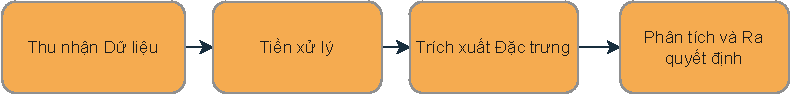
\includegraphics[width=0.8\textwidth]{vision_flow-crop.pdf}
    \caption{Pipeline CV: Thu nhận → Tiền xử lý → Trích xuất đặc trưng → Ra quyết định.}
\end{figure}
\end{frame}

% Slide 2: Bài toán CV cốt lõi
\begin{frame}{Bài toán CV cốt lõi}
\begin{itemize}
    \item Phân loại ảnh
    \item Phát hiện đối tượng (bounding box)
    \item Phân đoạn ảnh: ngữ nghĩa / thể hiện
    \item Ước lượng Tư thế Người (HPE) → keypoints
\end{itemize}
\end{frame}

% Slide 3: CNN + ViT
\begin{frame}{CNN \& Vision Transformer}
\begin{columns}[T]
\begin{column}{0.5\textwidth}
\textbf{CNN}: Tích chập + Pooling → học đặc trưng phân cấp
\begin{figure}
\centering
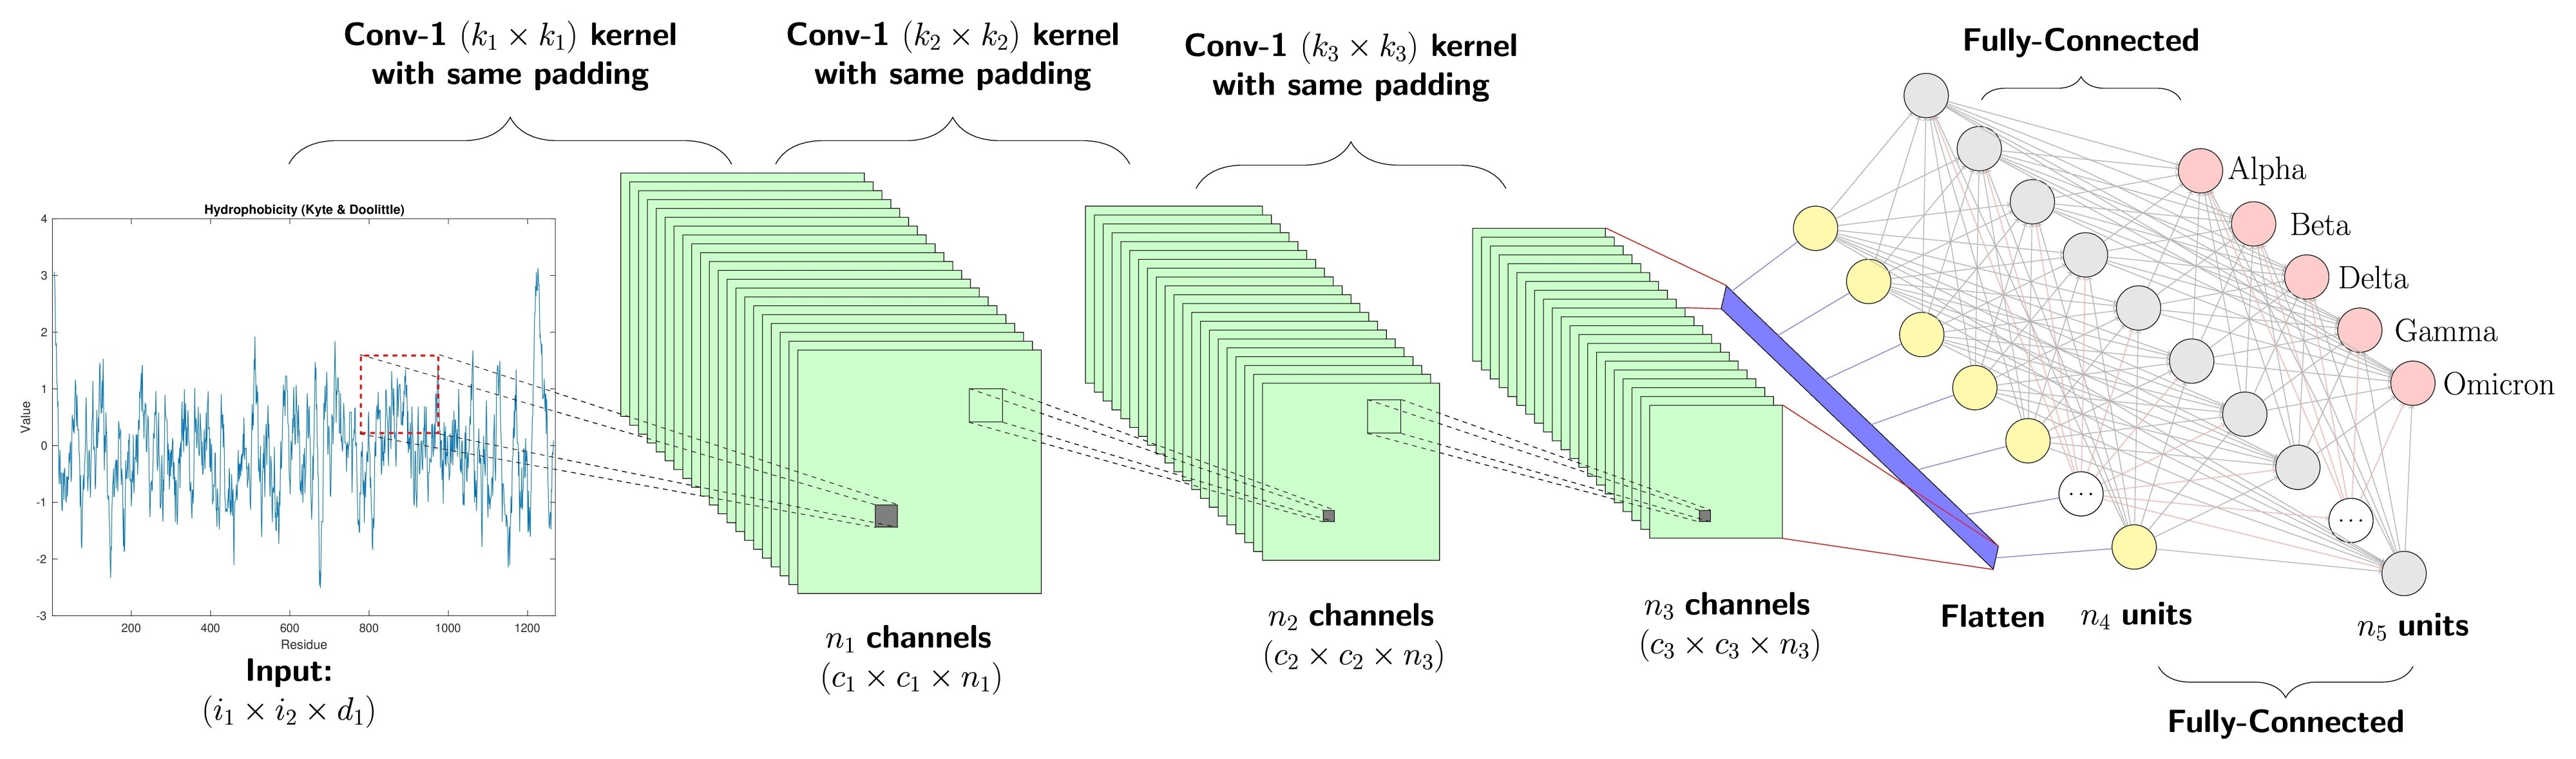
\includegraphics[width=0.9\textwidth]{2_2_convolution.jpeg}
\caption{CNN Operations}
\end{figure}
\end{column}
\begin{column}{0.5\textwidth}
\textbf{ViT}: Chia ảnh thành patches → Self-Attention → quan hệ toàn cục
\begin{figure}
\centering
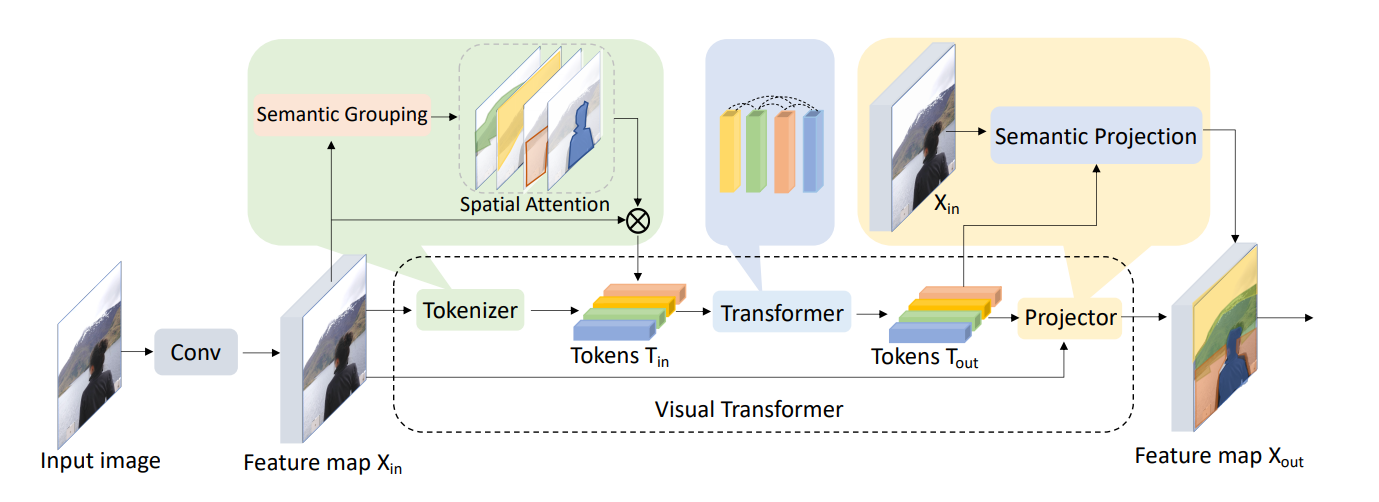
\includegraphics[width=0.9\textwidth]{visual_transformer.png}
\caption{Vision Transformer}
\end{figure}
\end{column}
\end{columns}
\end{frame}

% Slide 4: Datasets & Metrics - Detailed

\begin{frame}{Tập dữ liệu \& Metrics trong CV}
\begin{columns}[T]

% Column 1: Datasets
\begin{column}{0.55\textwidth}
\begin{block}{Tập dữ liệu chính}
\begin{itemize}
    \item \textbf{ImageNet} \cite{deng2009imagenet}: >14 triệu ảnh, ~20,000 nhãn. Chuẩn cho \textbf{phân loại ảnh}.
    \item \textbf{COCO} \cite{lin2014microsoft}: Hơn 330k ảnh, có \textbf{bounding box}, \textbf{segmentation}, \textbf{keypoints}. Chuẩn cho phát hiện đối tượng & phân đoạn.
    \item \textbf{MPII Human Pose}: ~25k ảnh, 16 keypoints trên cơ thể người. Chuẩn cho HPE.
    \item \textbf{COCO Keypoints}: Mở rộng COCO cho 17 keypoints, hỗ trợ HPE thời gian thực.
\end{itemize}
\end{block}
\end{column}

% Column 2: Metrics
\begin{column}{0.45\textwidth}
\begin{block}{Metrics}
\begin{itemize}
    \item IoU – Trùng khớp hộp giới hạn
    \item mAP – Hiệu suất phát hiện đối tượng
    \item F1-score – Trung bình điều hòa Precision & Recall
    \item OKS – Độ chính xác keypoints HPE
\end{itemize}
\end{block}
\end{column}

\end{columns}
\end{frame}

%mdeida pose edge---- HINH ANH MAU AN TOAN------------- edge

% Slide 1: Section Overview
\begin{frame}{Nhận diện Tư thế Người và Phát hiện Té ngã}
    \begin{block}{Tổng quan}
        Hệ thống tích hợp nhận diện tư thế (MediaPipe Pose) và phát hiện té ngã dựa trên đặc trưng động học/tư thế.
        \begin{itemize}
            \item Ứng dụng: Giám sát an toàn, phát hiện té ngã.
            \item Nền tảng: Thị giác máy tính thời gian thực.
        \end{itemize}
    \end{block}
\end{frame}

% Slide 2: Nhận diện Tư thế Người
\begin{frame}{Nhận diện Tư thế Người}
\begin{columns}[T]
    \begin{column}{0.45\textwidth}
        \centering
        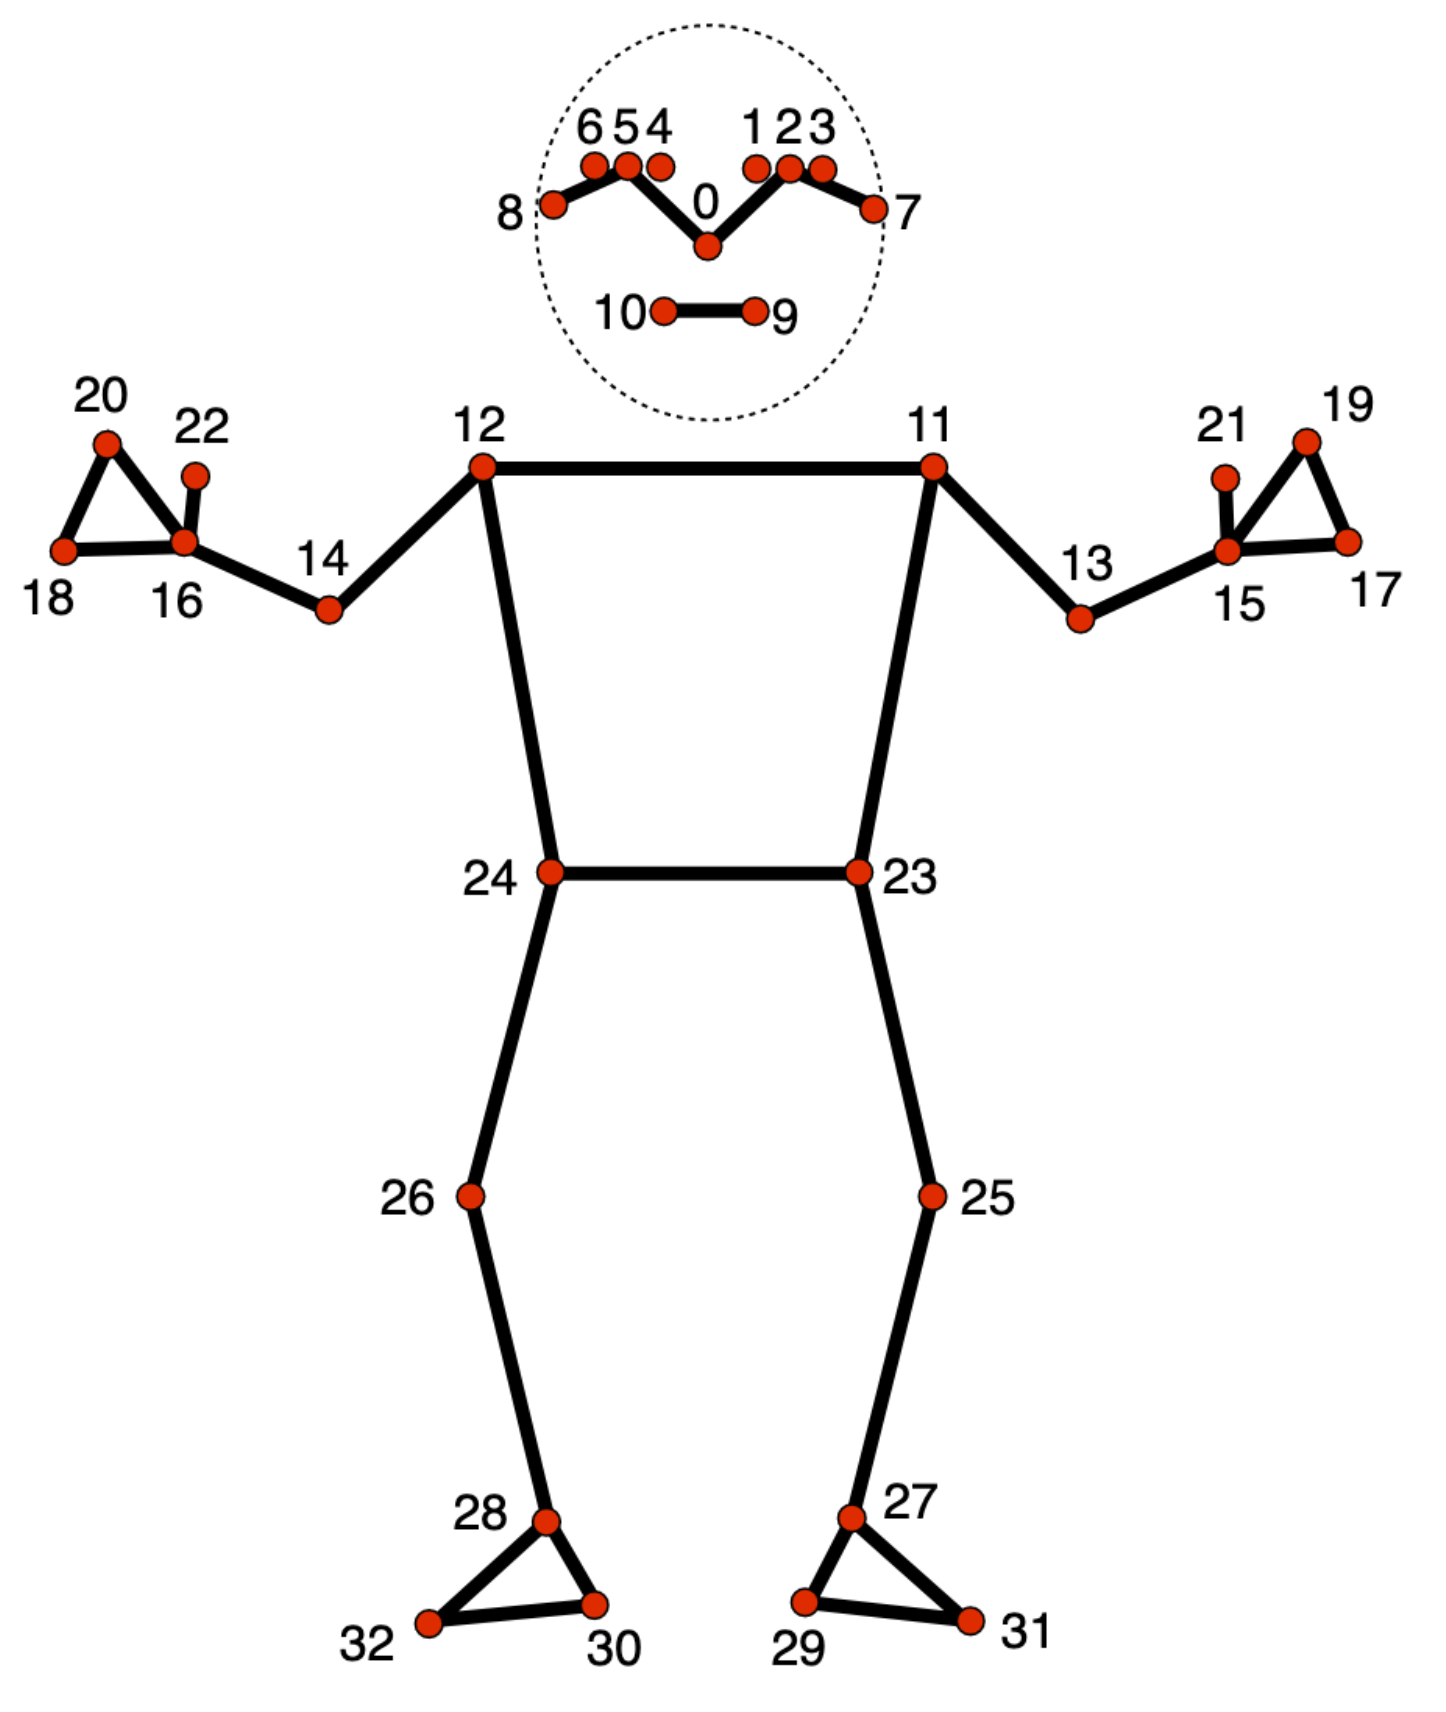
\includegraphics[height=0.8\textheight, keepaspectratio]{pose_landmarks_index.png}
        \vspace{0.2cm}
        {\small Keypoints cơ bản trong HPE (Human Pose Estimation).}
    \end{column}

    \begin{column}{0.55\textwidth}
        \begin{block}{Khái niệm}
            Ước lượng vị trí khớp từ hình ảnh/video:
            \[
                \mathcal{K} = \{k_i = (x_i, y_i, z_i, c_i)\}
            \]
            \small{\textit{($c_i$ là confidence score cho mỗi keypoint).}}
        \end{block}

        \begin{alertblock}{Phương pháp}
            \begin{itemize}
                \item \textbf{Top-down:} Phát hiện người trước, sau đó keypoints (MediaPipe).
                \item \textbf{Bottom-up:} Keypoints trước, nhóm thành người sau (OpenPose).
            \end{itemize}
        \end{alertblock}
    \end{column}
\end{columns}
\end{frame}

% Slide 3: MediaPipe Pose – Kiến trúc BlazePose
\begin{frame}{MediaPipe Pose – Kiến trúc BlazePose}
    \begin{block}{Kiến trúc BlazePose}
        BlazePose tối ưu HPE 3D với:
        \begin{itemize}
            \item \textbf{Nodes:} Các module xử lý tín hiệu hình ảnh.
            \item \textbf{Edges:} Luồng dữ liệu đồng bộ giữa các module.
        \end{itemize}
        \small{\textit{(Nodes = các bước tính toán; Edges = kết nối dữ liệu giữa các bước).}}
    \end{block}
\end{frame}

% Slide 4: MediaPipe Pose – Thành phần & Hậu xử lý
\begin{frame}{MediaPipe Pose – Thành phần & Hậu xử lý}
    \begin{exampleblock}{Thành phần chính}
        \begin{itemize}
            \item \textbf{Detection:} ROI từ ảnh RGB, phát hiện người.
            \item \textbf{Landmark:} 33 keypoints 3D, Loss: $\mathcal{L} = \sum \lambda_i \mathcal{L}_i$.
            \item \textbf{Tracking:} Dự đoán vị trí ROI cho khung tiếp theo.
        \end{itemize}
        \small{\textit{(Landmark 3D giúp đánh giá tư thế và động tác).}}
    \end{exampleblock}

    \begin{alertblock}{Hậu xử lý}
        \begin{itemize}
            \item \textbf{One Euro Filter:} Làm mịn nhiễu trong dữ liệu keypoints.
            \item \textbf{Chuẩn hóa $z$:} Dựa trên hông, tăng độ chính xác 3D.
        \end{itemize}
    \end{alertblock}
\end{frame}

% Slide 5: Thuật toán Phát hiện Té ngã
\begin{frame}{Thuật toán Phát hiện Té ngã}
    \begin{columns}[T]
        \column{0.5\textwidth}
        \begin{block}{Đặc trưng Động học}
            \begin{itemize}
                \item \textbf{Vận tốc COM:} $\vec{v}_{\text{COM}} = \frac{\Delta \vec{p}}{\Delta t}$
                \item \textbf{Gia tốc:} $a = \frac{\|\Delta \vec{v}\|}{\Delta t}$
            \end{itemize}
        \end{block}
        \begin{block}{Đặc trưng Tư thế}
            \begin{itemize}
                \item \textbf{AR (Aspect Ratio):} Tăng khi người nằm ngang
                \item \textbf{$\theta_{\text{body}}$:} Góc vai-hông
                \item \textbf{$\Delta h_{\text{head}}$:} Giảm chiều cao đầu
            \end{itemize}
            \small{\textit{(AR, $\theta$, $\Delta h$ giúp xác định tư thế bất thường).}}
        \end{block}

        \column{0.5\textwidth}
        \begin{alertblock}{Ba Giai đoạn Phát hiện}
            \begin{enumerate}
                \item \textbf{Sớm:} Tốc độ/gia tốc COM cao
                \item \textbf{Xác nhận:} AR, $\theta_{\text{body}}$ chỉ nằm ngang
                \item \textbf{Bất động:} Chuyển động $< M_{th}$
            \end{enumerate}
        \end{alertblock}
    \end{columns}
\end{frame}

% Ly thuyet de chuan bi cho viec xay dung phan cung 



% Slide 1: Kiến trúc Hệ thống
\begin{frame}{Kiến trúc Hệ thống Phát hiện Té ngã}
\begin{columns}[T]
\column{0.5\textwidth}
\begin{block}{Phân loại}
\begin{itemize}
    \item Camera-based
    \item Wearable-based
\end{itemize}
\end{block}
\column{0.5\textwidth}
\begin{block}{Thành phần chính}
\begin{enumerate}
    \item Thiết bị thu thập (IMU/Camera)
    \item Máy chủ xử lý (Deep Learning)
    \item Truyền thông (Wi-Fi, 4G)
\end{enumerate}
\end{block}
\end{columns}
\end{frame}

% Slide 2: Edge Processing
\begin{frame}{Xử lý Cục bộ (Edge)}
\begin{itemize}
    \item \textbf{ESP32}: lõi kép, FreeRTOS, xử lý song song.
    \item \textbf{IMU}: 
    \begin{itemize}
        \item Gia tốc kế, Con quay, Từ kế
        \item Sensor Fusion (Kalman/Madgwick)
    \end{itemize}
    \item \textbf{Ngưỡng phát hiện té ngã}:
    \[
    \|\mathbf{a}\| > a_{\text{shock}}, \quad \|\mathbf{a}\| \approx 1g
    \]
    \item \textbf{GPS}: định vị NMEA, hỗ trợ cứu hộ.
\end{itemize}
\end{frame}

% Slide 3: Host/Cloud Processing
\begin{frame}{Xử lý Máy chủ (Host/Cloud)}
\begin{columns}[T]
\column{0.5\textwidth}
\begin{block}{Camera Input}
ESP32-S3 + OV5640 (5MP) \\
→ stream JPEG qua Wi-Fi
\end{block}
\column{0.5\textwidth}
\begin{block}{Máy chủ}
\begin{itemize}
    \item GPU (Jetson Nano, Cloud)
    \item TensorFlow/PyTorch + OpenCV
    \item Đồng bộ IMU (MQTT/JSON) + Camera (JPEG)
\end{itemize}
\end{block}
\end{columns}
\end{frame}

% Slide 4: Truyền thông & Dự phòng
\begin{frame}{Hệ thống Truyền thông \& Dự phòng}
\begin{block}{Kênh truyền}
\begin{itemize}
    \item Wi-Fi: kênh chính
    \item 4G/LTE (EC800K): dự phòng, SMS/cuộc gọi khẩn
\end{itemize}
\end{block}

\begin{alertblock}{Logic vận hành}
\begin{enumerate}
    \item ESP32 phát hiện sơ cấp
    \item Truyền dữ liệu: Wi-Fi $\to$ 4G
    \item Server xác minh (IMU + HPE)
    \item Kích hoạt cảnh báo
\end{enumerate}
\end{alertblock}
\end{frame}

% Slide 5: Môi trường Phát triển
\begin{frame}{Môi trường Phát triển Phần mềm}
\begin{block}{ESP-IDF Framework}
\begin{itemize}
    \item Hỗ trợ FreeRTOS (đa nhiệm, lõi kép)
    \item Low-level Access (I2C/SPI, MQTT/HTTP tối ưu)
    \item Chuyên nghiệp hơn Arduino IDE
\end{itemize}
\end{block}
\end{frame}

% Section 1
\section{Tổng quan Kiến trúc Hệ thống}

\begin{frame}{Tổng quan Kiến trúc Hệ thống Phát hiện Té ngã}
\begin{block}{Phân loại hệ thống}
Hệ thống phát hiện té ngã hiện đại được chia thành hai nhóm chính:
\begin{itemize}
\item \textbf{Hệ thống dựa trên Camera}
\item \textbf{Hệ thống dựa trên Thiết bị đeo}
\end{itemize}
\end{block}

\begin{block}{Ba thành phần cốt lõi}
\begin{enumerate}
\item \textbf{Thiết bị Thu thập Dữ liệu}: Thu thập dữ liệu chuyển động (IMU) và/hoặc hình ảnh (Camera)
\item \textbf{Máy chủ Xử lý}: Thực hiện các thuật toán học sâu và logic ra quyết định phức tạp
\item \textbf{Hệ thống Truyền thông}: Đảm bảo luồng dữ liệu hai chiều và kích hoạt cảnh báo
\end{enumerate}
\end{block}
\end{frame}

% Section 2
\section{Vi điều khiển và Cảm biến}

\begin{frame}{Vi điều khiển ESP32}
\begin{columns}
\column{0.6\textwidth}
\begin{block}{Tại sao chọn ESP32?}
\begin{itemize}
\item Kiến trúc \textbf{lõi kép Xtensa LX6}
\item Xử lý song song hiệu quả
\item Tích hợp Wi-Fi, Bluetooth
\item Hỗ trợ giao thức MQTT, HTTP
\end{itemize}
\end{block}

\begin{block}{Phân công nhiệm vụ}
\begin{itemize}
\item \textbf{Lõi 1}: Xử lý thời gian thực (IMU, Kalman Filter)
\item \textbf{Lõi 2}: Truyền thông không dây
\end{itemize}
\end{block}

\column{0.4\textwidth}
\begin{center}
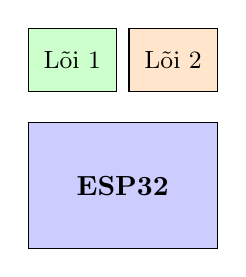
\begin{tikzpicture}[scale=0.8]
\draw[fill=blue!20] (0,0) rectangle (3,2);
\node at (1.5,1) {\textbf{ESP32}};
\draw[fill=green!20] (0,2.5) rectangle (1.4,3.5);
\node at (0.7,3) {\small Lõi 1};
\draw[fill=orange!20] (1.6,2.5) rectangle (3,3.5);
\node at (2.3,3) {\small Lõi 2};
\end{tikzpicture}
\end{center}
\end{columns}
\end{frame}

\begin{frame}{Cảm biến IMU}
\begin{block}{IMU (Inertial Measurement Unit)}
Tích hợp ba loại cảm biến quan trọng:
\end{block}

\begin{columns}
\column{0.33\textwidth}
\begin{alertblock}{Gia tốc kế}
\begin{itemize}
\item Đo gia tốc tuyến tính
\item Hiệu chuẩn từ số nguyên sang đơn vị $g$
\item Vector 3D: $\mathbf{a} = [a_x, a_y, a_z]$
\end{itemize}
\end{alertblock}

\column{0.33\textwidth}
\begin{alertblock}{Con quay hồi chuyển}
\begin{itemize}
\item Đo tốc độ góc
\item Dựa trên hiệu ứng Coriolis
\item Vector 3D: $\boldsymbol{\omega} = [\omega_x, \omega_y, \omega_z]$
\end{itemize}
\end{alertblock}

\column{0.33\textwidth}
\begin{alertblock}{Từ kế}
\begin{itemize}
\item Tham chiếu hướng từ trường
\item Hiệu chỉnh sai số trôi
\item Sensor Fusion (Madgwick, Kalman)
\end{itemize}
\end{alertblock}
\end{columns}
\end{frame}

\begin{frame}{Thuật toán Phát hiện Té ngã}
\begin{block}{Phát hiện dựa trên ngưỡng IMU}
Phân tích sự thay đổi đột ngột của gia tốc và tốc độ góc
\end{block}

\begin{columns}
\column{0.5\textwidth}
\begin{alertblock}{Shock Event}
Gia tốc tổng vượt ngưỡng cao:
$$\|\mathbf{a}\| > a_{\text{shock}}$$

Với: $$\|\mathbf{a}\| = \sqrt{a_x^2 + a_y^2 + a_z^2}$$
\end{alertblock}

\column{0.5\textwidth}
\begin{alertblock}{Post-fall State}
\begin{itemize}
\item Gia tốc tổng giảm về gần 1g
\item Biểu thị trạng thái nằm ngang
\item Tốc độ góc có thay đổi lớn
\end{itemize}
\end{alertblock}
\end{columns}

\vspace{0.5cm}
\begin{exampleblock}{Cảm biến GPS}
Module GPS (u-blox NEO-6M) sử dụng \textbf{đo tam giác} từ ít nhất 4 vệ tinh, cung cấp tọa độ cho dịch vụ cứu hộ khẩn cấp.
\end{exampleblock}
\end{frame}

% Section 3
\section{Hệ thống Camera và Xử lý}

\begin{frame}{Hệ thống Camera và Máy chủ}
\begin{columns}
\column{0.5\textwidth}
\begin{block}{Camera Input}
\begin{itemize}
\item ESP32-S3 + OV5640 5MP
\item Nén JPEG
\item Truyền qua Wi-Fi (RTSP/HTTP)
\item Xác minh hình ảnh
\end{itemize}
\end{block}

\begin{block}{Luồng dữ liệu}
\begin{itemize}
\item Luồng JSON/MQTT (IMU)
\item Luồng JPEG (Camera)
\item Đồng bộ hóa dữ liệu
\item Giảm báo động giả
\end{itemize}
\end{block}

\column{0.5\textwidth}
\begin{block}{Kiến trúc Máy chủ}
\textbf{Phần cứng:}
\begin{itemize}
\item AWS, Google Cloud
\item NVIDIA Jetson Nano
\item GPU cho tính toán Tensor
\end{itemize}

\textbf{Phần mềm:}
\begin{itemize}
\item TensorFlow/PyTorch
\item OpenCV
\item Thuật toán HPE
\item Học sâu
\end{itemize}
\end{block}
\end{columns}
\end{frame}

% Section 4
\section{Hệ thống Truyền thông}

\begin{frame}{Module Truyền thông}
\begin{columns}
\column{0.5\textwidth}
\begin{alertblock}{Wi-Fi (ESP32) - Kênh chính}
\begin{itemize}
\item Truyền tải dữ liệu dung lượng lớn
\item Video/hình ảnh
\item Giao tiếp MQTT với máy chủ
\item Độ trễ thấp
\end{itemize}
\end{alertblock}

\column{0.5\textwidth}
\begin{alertblock}{4G/LTE (EC800K) - Dự phòng}
\begin{itemize}
\item Hoạt động khi Wi-Fi không khả dụng
\item Hỗ trợ định vị GPS
\item Cuộc gọi khẩn cấp tự động
\item SMS cảnh báo qua AT commands
\end{itemize}
\end{alertblock}
\end{columns}
\end{frame}

\begin{frame}{Logic Hoạt động}
\begin{enumerate}
\item \textbf{Thu thập/Xử lý Sơ cấp}
\begin{itemize}
\item ESP32 thu thập dữ liệu IMU/Camera
\item Phát hiện té ngã dựa trên ngưỡng IMU
\end{itemize}

\item \textbf{Quyết định Truyền thông}
\begin{itemize}
\item Nếu phát hiện té ngã → truyền dữ liệu lên máy chủ
\item Ưu tiên Wi-Fi, dự phòng 4G
\end{itemize}

\item \textbf{Xác minh Máy chủ}
\begin{itemize}
\item Phân tích hình ảnh (HPE)
\item Kết hợp dữ liệu IMU
\item Multi-stage Fall Detection Logic
\end{itemize}

\item \textbf{Kích hoạt Cảnh báo}
\begin{itemize}
\item Xác nhận té ngã → ra lệnh cho ESP32
\item Kích hoạt Module EC800K gửi SMS/Cuộc gọi
\end{itemize}
\end{enumerate}
\end{frame}

% Section 5
\section{Môi trường Phát triển}

\begin{frame}{ESP-IDF Framework}
\begin{block}{Tại sao chọn ESP-IDF thay vì Arduino IDE?}
\end{block}

\begin{columns}
\column{0.5\textwidth}
\begin{alertblock}{Hỗ trợ RTOS}
\begin{itemize}
\item Tích hợp FreeRTOS
\item Tận dụng kiến trúc lõi kép
\item Đa nhiệm thực sự
\item Tác vụ IMU song song với Wi-Fi
\end{itemize}
\end{alertblock}

\column{0.5\textwidth}
\begin{alertblock}{Truy cập Cấp thấp}
\begin{itemize}
\item Truy cập trực tiếp thanh ghi phần cứng
\item Cấu hình chi tiết cảm biến (I2C/SPI)
\item Tối ưu hóa giao thức mạng
\item Hiệu suất thời gian thực
\end{itemize}
\end{alertblock}
\end{columns}
\end{frame}
